\section{Three Examples of Convergence} \label{sec:1}
\subsection{Convergence in $\mathbb{R}$}
Let $(x_n)$ be a sequence in $\mathbb{R}$ and $x \in \mathbb{R}$.
We say $(x_n)$ \textit{converges} to $x$ and write $x_n \to x$ if
\begin{align*}
    \forall \; \epsilon > 0 \quad \exists \; N \quad \forall \; n \geq N \quad |x_n - x| < \epsilon.
\end{align*} 
Useful fact: $\forall \; a, b \in \mathbb{R} \ |a+b| \leq |a| + |b|$ (Triangle Inequality).

Bolzano-Weierstrass Theorem (BWT)
A bounded sequence in $\mathbb{R}$ must have a convergent subsequence (Proof by interval bisection).

Recall: A sequence $(x_n)$ in $\mathbb{R}$ is Cauchy if 
\begin{align*}
    \forall \; \epsilon > 0 \quad \exists \; N \quad \forall \; m, n \geq N \quad |x_m - x_n| < \epsilon.
\end{align*} 

\begin{exercise}[Easy]
    Show convergent $\implies$ Cauchy.
\end{exercise} 

General Principle of Convergence (GPC)
Any Cauchy sequence in $\mathbb{R}$ converges.

\begin{proof}[Outline]
    If $(x_n)$ Cauchy then $(x_n)$ bounded so by BWT has a convergent subsequence, say $x_{n_j} \to x$.
    But as $(x_n)$ Cauchy, $x_n \to x$.
\end{proof} 

\subsection{Convergence in $\mathbb{R}^2$}
\begin{remark}
    This all works in $\mathbb{R}^n$
\end{remark} 

Let $(z_n)$ be a sequence in $\mathbb{R}^2$ and $z \in \mathbb{R}^2$.
What should $z_n \to z$ mean?

In $\mathbb{R}$: ``As $n$ gets large, $z_n$ gets arbitrarily close to $z$.''

What does `close' mean in $\mathbb{R}^2$?

In $\mathbb{R}$: $a, b$ close if $|a - b|$ small.
In $\mathbb{R}^2$: Replace $|\cdot|$ by $\left \lVert \cdot \right \rVert $

Recall: If $z = (x, y)$ then $\left \lVert z \right \rVert = \sqrt{x^2 + y^2}$.

Triangle Inequality If $a, b \in \mathbb{R}^2$ then $\left \lVert a + b \right \rVert \leq \left \lVert a \right \rVert + \left \lVert b \right \rVert$.

\begin{definition}
    Let $(z_n)$ be a sequence in $\mathbb{R}^2$ and $z \in \mathbb{R}^2$.
    We say $(z_n)$ \vocab{converges} to $z$ and write $z_n \to z$ if $\forall \; \epsilon > 0 \ \exists \; N \ \forall \; n \geq N \ \left \lVert z_n - z \right \rVert < \epsilon$. 

    Equivalently, $z_n \to z$ iff $\left \lVert z_n - z \right \rVert \to 0$ (convergence in $\mathbb{R}$).
\end{definition} 

\begin{example}
    Let $(z_n), (w_n)$ be sequences in $\mathbb{R}^2$ with $z_n \to z, w_n \to w$. 
    Then $z_n + w_n \to z + w$.
\end{example} 

\begin{proof}
    \begin{align*}
        \left \lVert (z_n + w_n) - (z + w) \right \rVert &\leq \left \lVert z_n - z \right \rVert + \left \lVert w_n - w \right \rVert \\
        &\to 0 + 0 = 0 \ \text{(by results from IA)}.
    \end{align*} 
\end{proof} 

In fact, given convergence in $\mathbb{R}$, convergence in $\mathbb{R}^2$ is easy:
\begin{proposition} \label{prop:one}
    Let $(z_n)$ be a sequence in $\mathbb{R}^2$ and let $z \in \mathbb{R}^2$.
    Write $z_n = (x_n, y_n)$ and $z = (x, y)$.
    Then $z_n \to z$ iff $x_n \to x$ and $y_n \to y$.
\end{proposition} 

\begin{proof}
    ($\implies$): $|x_n - x|, |y_n - y| \leq \norm{z_n - z}$.
    So if $\norm{z_n - z} \to 0$ then $|x_n - x| \to 0$ and $|y_n - y| \to 0$.

    ($\Longleftarrow$): If $|x_n - x| \to 0$ and $|y_n - y| \to 0$ then $\norm{z_n - z} = \sqrt{(x_n - x)^2 + (y_n - y)^2} \to 0$ by results in $\mathbb{R}$.
\end{proof} 

\begin{definition}[Bounded Sequence]
    A sequence $(z_n)$ in $\mathbb{R}^2$ is \vocab{bounded} if $\exists \; M \in \mathbb{R}$ s.t. $\forall \; n \ \norm{z_n} \leq M$.
\end{definition} 

\begin{theorem}[BWT in $\mathbb{R}^2$]
    A bounded sequence in $\mathbb{R}^2$ must have a convergent subsequence.
\end{theorem} 

\begin{theorem}[GPC for $\mathbb{R}^2$]
    Any Cauchy sequence in $\mathbb{R}^2$ converges.
\end{theorem} 

\begin{proof}
    Let $(z_n)$ be a Cauchy sequence in $\mathbb{R}^2$.
    Write $z_n = (x_n, y_n)$.
    For all $m, n, |x_m - x_n| \leq \norm{z_m - z_n}$ so $(x_n)$ is a Cauchy sequence in $\mathbb{R}$, so converges by GPC.
    Similarly, $(y_n)$ converges in $\mathbb{R}$.
    So by \ref{prop:one}, $(z_n)$ converges.
\end{proof} 

\underline{Thought for the day} What about continuity?
Let $f: \mathbb{R}^2 \to \mathbb{R}$.
What does it mean for $f$ to be continuous?
(Simple modification of defn for $\mathbb{R} \to \mathbb{R}$).

What can we do with it?

Big theorem in IA: If $f: \mathbb{R} \to \mathbb{R}$ is a continuous function on a closed bounded interval then $f$ is bounded and attains its bounds.

Is there a similar theorem for $\mathbb{R}^2 \to \mathbb{R}$.
What do we replace `closed bounded interval' by?
We proved the theorem using BWT.
Why did it work?
Why did we need a closed bounded interval to make it work?
What can we do in $\mathbb{R}^2$?

\subsection{Convergence of Functions}
Let $X \subset \mathbb{R}$\footnote{Mostly can think of $X = \mathbb{R}$ or some interval}, let $f_n : X \to \mathbb{R}$ ($n \geq 1$) and let $f: X \to \mathbb{R}$.
What does it mean for $f_n$ to converge to $f$.

Obvious idea:
\begin{definition}[Pointwise convergence]
    Say $(f_n)$ \vocab{converges pointwise} to $f$ and write $f_n \to f$ pointwise if $\forall \; x \in X \ f_n(x) \to f(x)$ as $n \to \infty$.
\end{definition} 

Pros
\begin{itemize}
    \item Simple
    \item Easy to check
    \item Defined in terms of convergence in $\mathbb{R}$
\end{itemize} 
Cons
\begin{itemize}
    \item Doesn't preserve `nice' properties.
    \item `Doesn't feel right'.
\end{itemize} 

In all three examples, have $X = [0, 1], f_n \to f$ pointwise.

\begin{example}[Every $f_n$ continuous but $f$ not] ~\vspace*{-1.5\baselineskip}
    \begin{align*}
        f_n(x) &= \begin{cases}
            nx & x \leq \frac{1}{n} \\
            1 & x \geq \frac{1}{n}
        \end{cases} \\
        f(x) &= \begin{cases}
            0 & x= 0 \\
            1 & x> 0
        \end{cases} 
    \end{align*} 
    {\par
        \centering 
        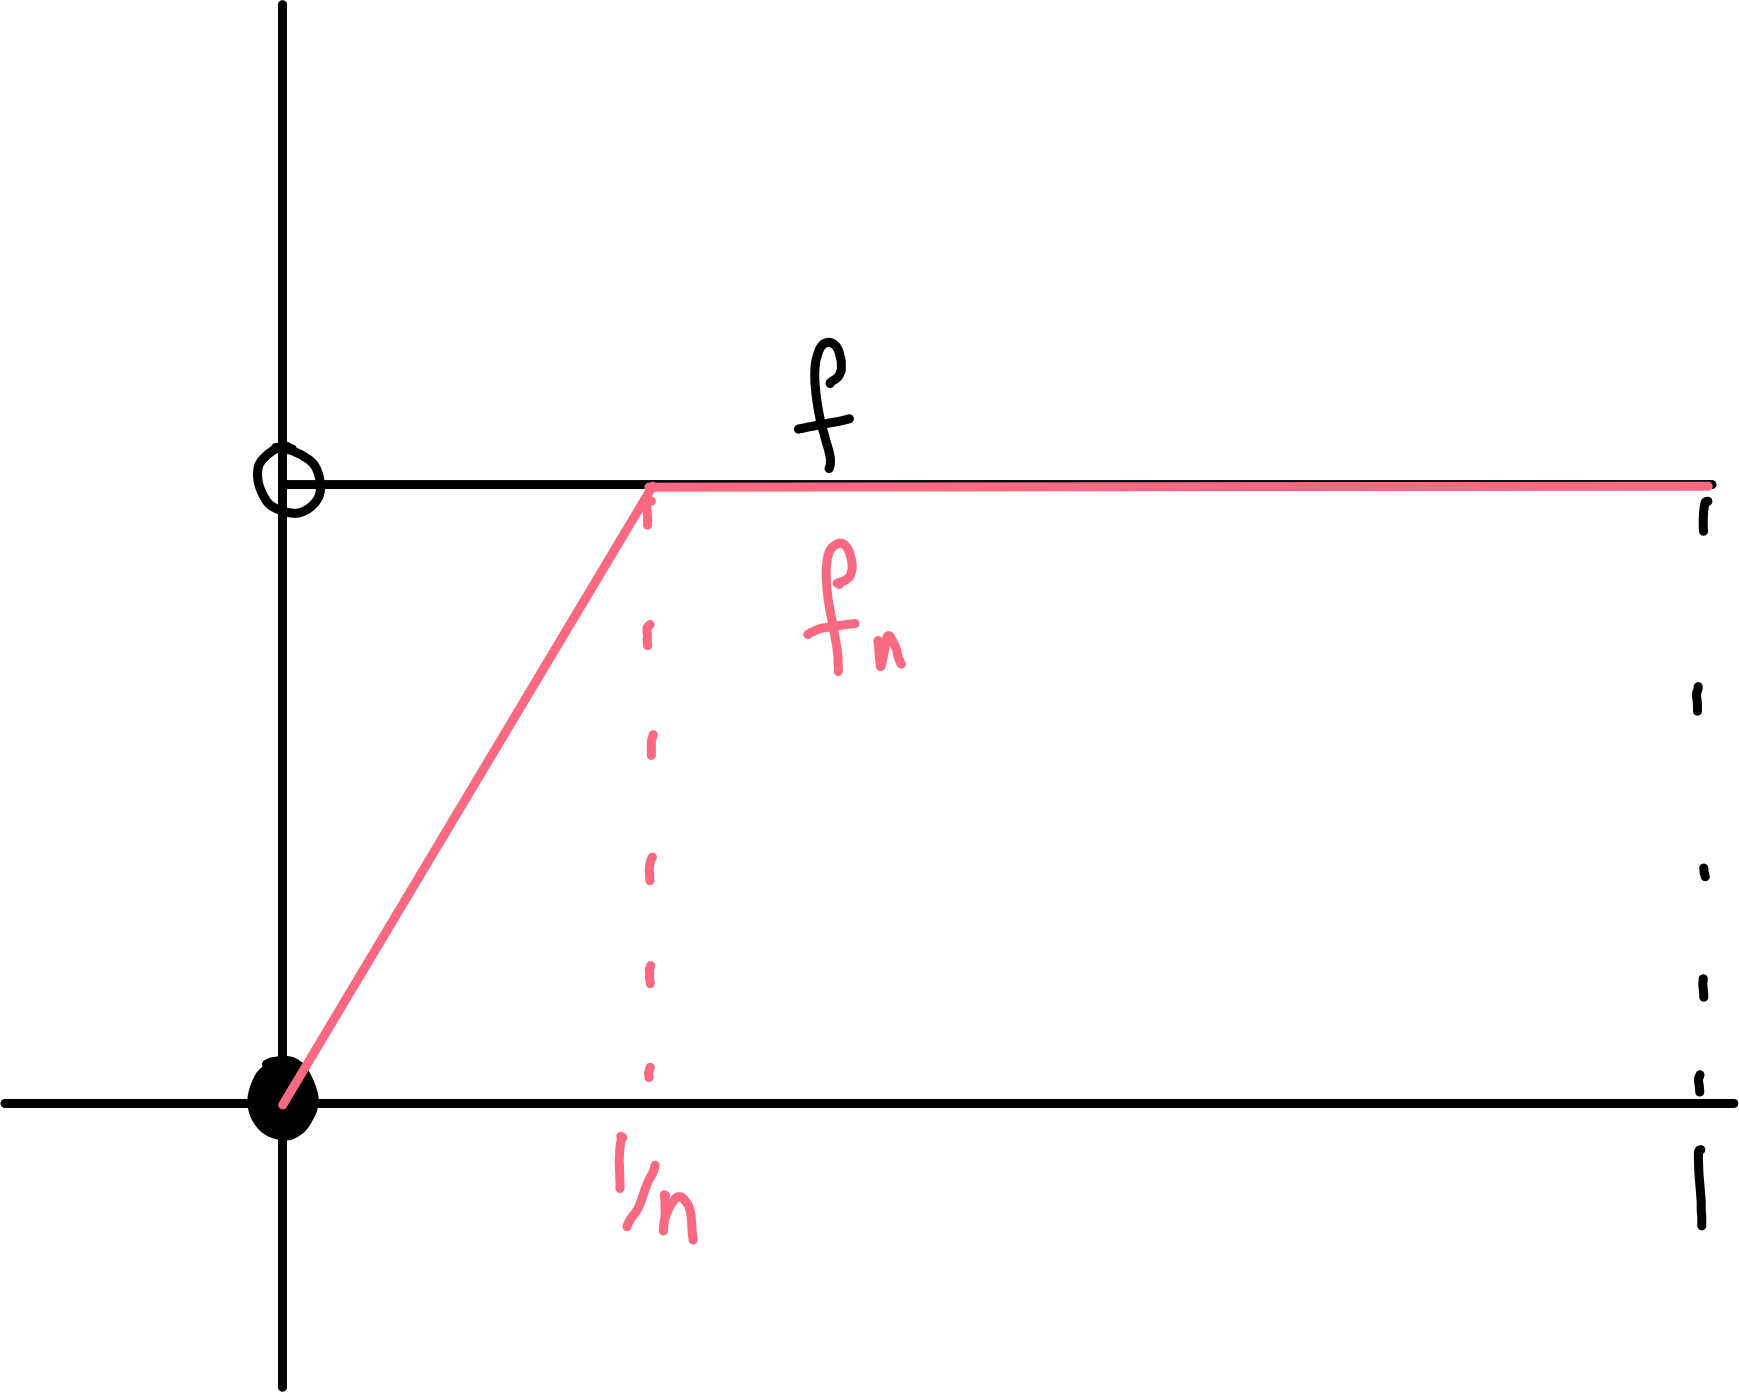
\includegraphics[height=5cm]{01-pointwise1} 
    \par}
    Clearly $f_n$ continuous for all $n$ but $f$ not.
    If $x = 0,\ \forall \; n \ f_n(0) = 0 = f(0)$.
    If $x > 0$, for sufficiently large $n$ $f_n(x) = 1 = f(x)$ so $f_n(x) \to f(x)$.
\end{example} 

\begin{example}[Every $f_n$ integrable but $f$ not]
    \begin{align*}
        f(x) &= \begin{cases}
            1 & x \in \mathbb{Q} \\
            0 & x \notin \mathbb{Q}
        \end{cases}.
    \end{align*} 
    This is a non integrable\footnote{N.B. As in IA `integrable' means `Riemann integrable'} function so now we want to find $f_n$ such that they converge pointwise to this.
    Enumerate the rationals in $[0, 1]$ as $q_1, q_2, \dots$
    For $n \geq 1$, set $f_n(x) = \mathbbm{1}_{q_1, \dots, q_n}$. 
    $f_n$ integrable as it is nonzero at finitely many points.
\end{example} 

\begin{example}[Every $f_n$ and $f$ integrable but $\int_0^1 f_n \not\to \int_0^1 f$]
Let $f(x) = 0$ for all $x$, so $\int_0^1 f = 0$.
Define $f_n$ s.t. $\int_0^1 f_n = 1$ for all $n$.
{\par
    \centering 
    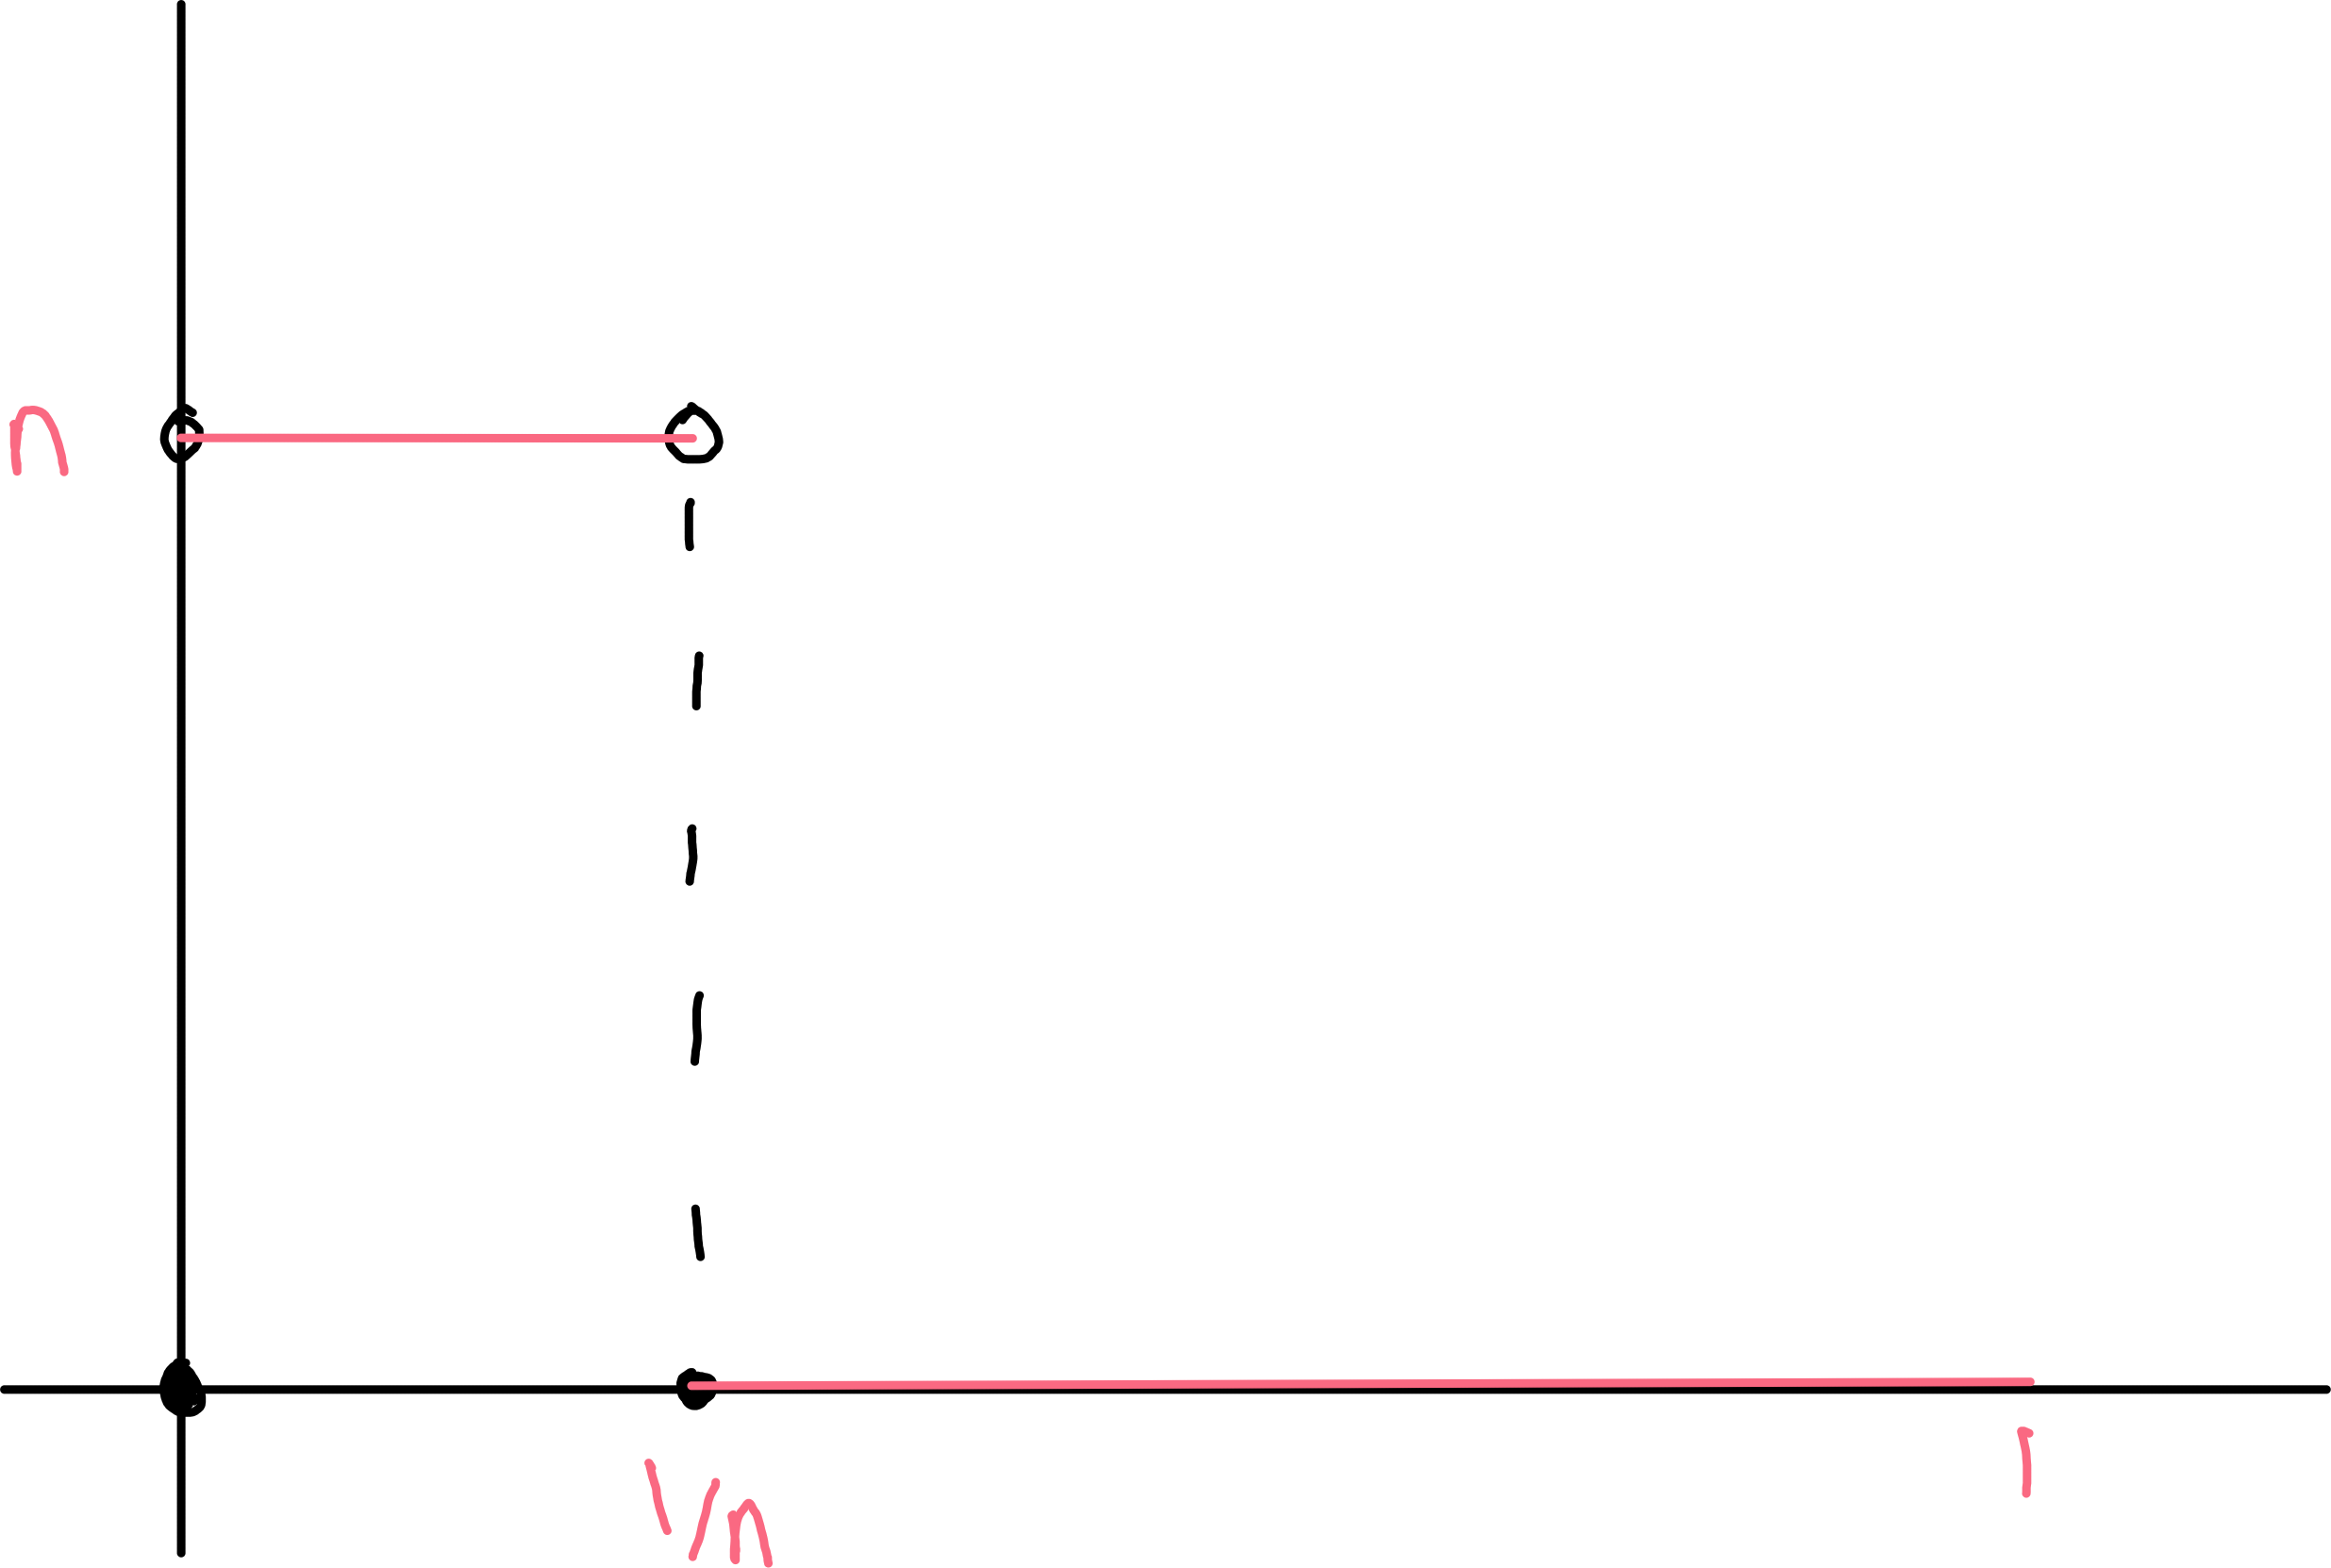
\includegraphics[height=5cm]{01-pointwise2} 
\par}
\begin{align*}
    f_n(x) &= \begin{cases}
        n & 0 < x < \frac{1}{n} \\
        0 & \text{otherwise}
    \end{cases}.
\end{align*} 
\end{example} 

Better definition:
\begin{definition}[Uniform convergence]
    Let $X \subset \mathbb{R}$, $f_n : X \to \mathbb{R}$ ($n \geq 1$), $f: X \to \mathbb{R}$.
    We say $(f_n)$ \vocab{converges uniformly} to $f$ and write $f_n \to f$ uniformly if $\forall \; \epsilon > 0 \ \exists \; N \ \forall \; x \in X \ \forall \; n \geq N \ |f_n(x) - f(x)| < \epsilon$.
\end{definition} 

cf $f_n \to f$ pointwise: $\forall \; \epsilon > 0 \ \forall \; x \in X \ \exists \; N \ \forall \; n \geq N \ |f_n(x) - f(x)| < \epsilon$. (We have swapped the $\forall \; x \in x$ and $\exists \; N$).
Pointwise convergence allows for $N$ to be a function of $x$ whilst uniform convergence requires $N$ to work for all $x$ even the worst case.
In particular, $f_n \to f$ uniformly $\implies f_n \to f$ pointwise.

\begin{center}
    \tikzset{every picture/.style={line width=0.75pt}} %set default line width to 0.75pt        

    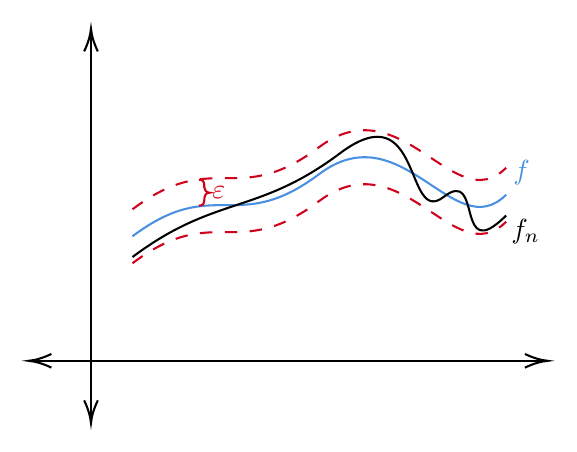
\begin{tikzpicture}[x=0.75pt,y=0.75pt,yscale=-1,xscale=1]
    %uncomment if require: \path (0,300); %set diagram left start at 0, and has height of 300
    
    %Straight Lines [id:da15070589522945865] 
    \draw    (120,42) -- (120,228) ;
    \draw [shift={(120,230)}, rotate = 270] [color={rgb, 255:red, 0; green, 0; blue, 0 }  ][line width=0.75]    (10.93,-3.29) .. controls (6.95,-1.4) and (3.31,-0.3) .. (0,0) .. controls (3.31,0.3) and (6.95,1.4) .. (10.93,3.29)   ;
    \draw [shift={(120,40)}, rotate = 90] [color={rgb, 255:red, 0; green, 0; blue, 0 }  ][line width=0.75]    (10.93,-3.29) .. controls (6.95,-1.4) and (3.31,-0.3) .. (0,0) .. controls (3.31,0.3) and (6.95,1.4) .. (10.93,3.29)   ;
    %Straight Lines [id:da06812433005878815] 
    \draw    (338,200) -- (92,200) ;
    \draw [shift={(90,200)}, rotate = 360] [color={rgb, 255:red, 0; green, 0; blue, 0 }  ][line width=0.75]    (10.93,-3.29) .. controls (6.95,-1.4) and (3.31,-0.3) .. (0,0) .. controls (3.31,0.3) and (6.95,1.4) .. (10.93,3.29)   ;
    \draw [shift={(340,200)}, rotate = 180] [color={rgb, 255:red, 0; green, 0; blue, 0 }  ][line width=0.75]    (10.93,-3.29) .. controls (6.95,-1.4) and (3.31,-0.3) .. (0,0) .. controls (3.31,0.3) and (6.95,1.4) .. (10.93,3.29)   ;
    %Curve Lines [id:da9975807479144934] 
    \draw [color={rgb, 255:red, 74; green, 144; blue, 226 }  ,draw opacity=1 ]   (140,140) .. controls (180,110) and (190,140) .. (230,110) .. controls (270,80) and (295,145) .. (320,120) ;
    %Curve Lines [id:da8386196196350342] 
    \draw [color={rgb, 255:red, 208; green, 2; blue, 27 }  ,draw opacity=1 ] [dash pattern={on 4.5pt off 4.5pt}]  (140,127) .. controls (180,97) and (190,127) .. (230,97) .. controls (270,67) and (295,132) .. (320,107) ;
    %Curve Lines [id:da7136000427009845] 
    \draw [color={rgb, 255:red, 208; green, 2; blue, 27 }  ,draw opacity=1 ] [dash pattern={on 4.5pt off 4.5pt}]  (140,153) .. controls (180,123) and (190,153) .. (230,123) .. controls (270,93) and (295,158) .. (320,133) ;
    %Shape: Brace [id:dp021850826872210183] 
    \draw  [color={rgb, 255:red, 208; green, 2; blue, 27 }  ,draw opacity=1 ] (172,125.25) .. controls (173.71,125.25) and (174.57,124.39) .. (174.57,122.68) -- (174.57,122.68) .. controls (174.57,120.23) and (175.43,119) .. (177.15,119) .. controls (175.43,119) and (174.57,117.77) .. (174.57,115.32)(174.57,116.43) -- (174.57,115.32) .. controls (174.57,113.61) and (173.71,112.75) .. (172,112.75) ;
    %Curve Lines [id:da39763918210258864] 
    \draw    (140,150) .. controls (180,120) and (200,130) .. (240,100) .. controls (280,70) and (271,135.75) .. (290,121) .. controls (309,106.25) and (295,155) .. (320,130) ;
    
    % Text Node
    \draw (177,119) node [anchor=west] [inner sep=0.75pt]  [color={rgb, 255:red, 208; green, 2; blue, 27 }  ,opacity=1 ]  {$\varepsilon $};
    % Text Node
    \draw (322,116.6) node [anchor=south west] [inner sep=0.75pt]  [color={rgb, 255:red, 74; green, 144; blue, 226 }  ,opacity=1 ]  {$f$};
    % Text Node
    \draw (321,130.4) node [anchor=north west][inner sep=0.75pt]  [color={rgb, 255:red, 0; green, 0; blue, 0 }  ,opacity=1 ]  {$f_{n}$};
    
    
    \end{tikzpicture}
    

\end{center}

Equivalently, $f_n \to f$ uniformly if for sufficiently large $n$ $f_n - f$ is bounded and $\sup_{x \in X} |f_n - f| \to 0$.

\begin{theorem}[A uniform limit of cts functions is cts] \label{thm:4}
    Let $X \subset \mathbb{R}$, let $f_n: X \to \mathbb{R}$ be continuous ($n \geq 1$) and let $f_n \to f: X \to \mathbb{R}$ uniformly.
    Then $f$ is cts.
\end{theorem} 

\begin{proof}
    Let $x \in X$.
    Let $\epsilon > 0$.
    As $f_n \to f$ uniformly, we can find $N$ s.t. $\forall \; n \geq N \ \forall \; y \in X \ |f_n(y) - f(y)| < \epsilon$.
    In particular, $\forall \; y \in X \ |f_N(y) - f(y)| < \epsilon$.
    As $f_N$ is cts, we can find $\delta > 0$ s.t. $\forall \; y \in X,\ |y - x| < \delta \implies |f_N(y) - f_N(x)| < \epsilon$.
    Now let $y \in X$ with $|y - x| < \delta$.
    Then
    \begin{align*}
        |f(y) - f(x)| &\leq |f(y) - f_N(y)| + |f_N(y) - f_N(x)| + |f_N(x) - f(x)|\footnote{The core of this proof is this inequality.} \\
        &< \epsilon + \epsilon + \epsilon = 3\epsilon.
    \end{align*} 
    Hence $f$ is cts.
\end{proof} 

\begin{remark}
    This is often called a `$3\epsilon$ proof' (or an $\frac{\epsilon}{3}$ proof).
\end{remark} 

\begin{theorem} \label{thm:5}
    Let $f_n: [a, b] \to \mathbb{R}$ ($n \geq 1$) be integrable and let $f_n \to f: [a, b] \to \mathbb{R}$ uniformly.
    Then $f$ is integrable and $\int_a^b f_n \to \int_a^b f$ as $n \to \infty$.
\end{theorem} 

\begin{proof}
    As $f_n \to f$ uniformly, we can pick $n$ suff. large s.t. $f_n - f$ is bounded.
    Also $f_n$ is bounded (as integrable).
    So by triangle inequality, $f = (f - f_n) + f_n$ is bounded.
    Let $\epsilon > 0$.
    As $f_n \to f$ uniformly there is some $N$ s.t. $\forall \; n \geq N \ \forall \; x \in [a, b]$ we have $|f_n(x) - f(x)| < \epsilon$. \\
    In particular, $\forall \; x \in [a, b] \ |f_N(x) - f(x)| < \epsilon$.

    By Riemann's criterion, there is some dissection $\mathcal{D}$ of $[a, b]$ for which $S(f_n, \mathcal{D}) - s(f_n, \mathcal{D}) < \epsilon$.
    Let $\mathcal{D} = \{x_0, x_1, x_2, \dots, x_k\}$ where $a = x_0 < x_1 < \dots < x_k = b$.
    Now \begin{align*}
        S(f, \mathcal{D}) &= \sum_{i=1}^{k}  (x_i - x_{i-1}) \sup_{x \in [x_{i-1}, x_i]} f(x) \\
        &\leq \sum_{i=1}^{k}  (x_i - x_{i-1}) \sup_{x \in [x_{i-1}, x_i]} (f_N(x) + \epsilon) \\
        &= \sum_{i=1}^{k}  (x_i - x_{i-1}) \left( \left( \sup_{x \in [x_{i-1}, x_i]} f_N(x) \right) + \epsilon\right) \\
        &= \sum_{i=1}^{k}  (x_i - x_{i-1}) \sup_{x \in [x_{i-1}, x_i]} f_N(x) + \sum_{i=1}^{k} (x_i - x_{i-1}) \epsilon \\
        &= S(f_N, \mathcal{D}) + (b - a)\epsilon.
    \end{align*} 
    That is $S(f, \mathcal{D}) \leq S(f_N, \mathcal{D}) + (b - a)\epsilon$.
    Similarly $s(f, \mathcal{D}) \geq s(f_N, \mathcal{D}) - (b - a)\epsilon$.
    Hence
    \begin{align*}
        S(f, \mathcal{D}) - s(f, \mathcal{D}) &\leq S(f_N, \mathcal{D}) - s(f_N, \mathcal{D}) + 2(b - a) \epsilon \\
        &< (2(b-a) + 1) \epsilon
    \end{align*} 
    But $2(b-a) + 1$ is a constant so $(2(b-a) + 1) \epsilon$ can be made arbitrarily small.
    Hence by Riemann's criterion, $f$ is integrable over $[a, b]$.

    Now, for any $n$ suff. large that $f_n - f$ is bounded, 
    \begin{align*}
        \left| \int_a^b f_n - \int_a^b f \right| &= \left| \int_a^b (f_n - f) \right| \\
        &\leq \int_a^b |f_n - f| \\
        &\leq (b - a) \sup_{x \in [a, b]} |f_n - f| \\
        &\to 0 \text{ as } n \to \infty \text{ since $f_n \to f$ uniformly.}\footnote{Note we said that $f_n \to f$ uniformly if $\sup |f_n - f| \to 0$.}
    \end{align*} 
\end{proof} 

What about differentiation?
Here even uniform convergence isn't enough.

\begin{example}
    $f_n : (-1, 1) \to \mathbb{R}$, each $f_n$ differentiable, $f_n \to f$ uniformly, $f$ not diff.

    Let $f(x) = |x|$ which is not differentiable at $0$.
    {\par \centering 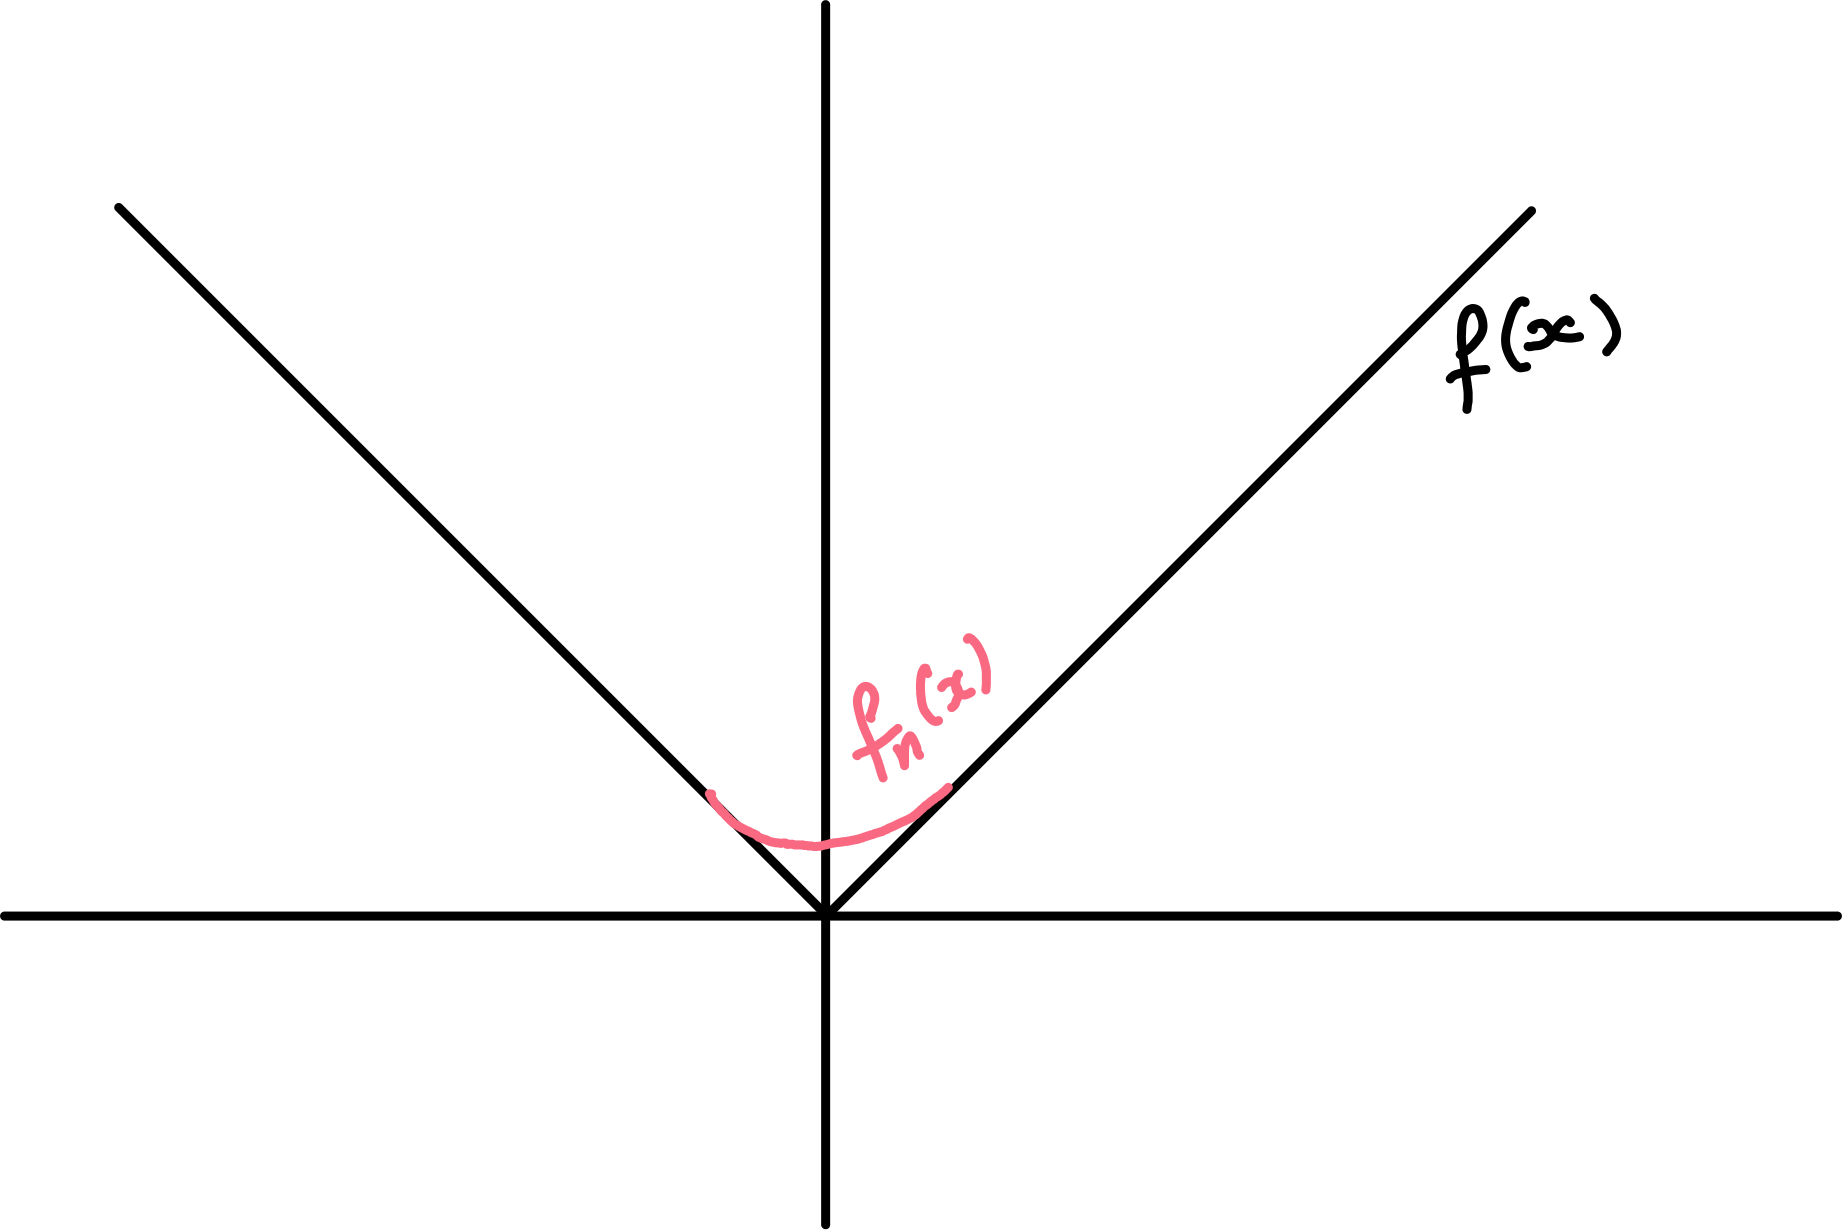
\includegraphics[height=5cm]{01-modx} \par}

    \begin{align*}
        f_n &= \begin{cases}
            |x| & |x| \geq \frac{1}{n} \\
            ax^2 + bx + c & |x| < \frac{1}{n}
        \end{cases}.
    \end{align*} 
    We need $a(\frac{1}{n})^2 + \frac{b}{n} + c = \frac{1}{n}$ for continuity.
    Thus $b = 0$ and $c = \frac{1}{n} - \frac{a}{n^2}$.

    Also need $2a \frac{1}{n} + b = 1$ and $2a (- \frac{1}{n}) = -1$ for differentiability so take $a = \frac{n}{2}$, $c = \frac{1}{n} - \frac{1}{2n} = \frac{1}{2n}$.

    If $|x| \geq \frac{1}{n}$ then $|f_n(x) - f(x)| = 0$.
    If $|x| < \frac{1}{n}$:
    \begin{align*}
        |f_n(x) - f(x)| &= \left| \frac{n}{2} x^2 + \frac{1}{2n} - |x| \right| \\
        &\leq \frac{n}{2} x^2 + \frac{1}{2n} + |x| \\
        &\leq \frac{n}{2} (\frac{1}{n})^2 + \frac{1}{2n} + \frac{1}{n} \\
        &= \frac{1}{2n} + \frac{1}{2n} + \frac{1}{n} \\
        &= \frac{2}{n}
    \end{align*} 
    So $\sup_{x \in (-1, 1)} |f_n(x) - f(x)| \leq \frac{2}{n} \to 0$ as $n \to \infty$.
    So $f_n \to f$ uniformly.
\end{example} 

If fact we need uniform convergence of the derivatives.

\begin{theorem} \label{thm:6}
    Let $f_n : (u, v) \to \mathbb{R}$ ($n \geq 1$) with $f_n \to f : (u, v) \to \mathbb{R}$ pointwise.
    Suppose further each $f_n$ is continuously differentiable and that $f_n' \to g : (u, v) \to \mathbb{R}$ uniformly.
    Then $f$ is differentiable with $f' = g$.
\end{theorem} 

\begin{proof}
    Fix $a \in (u, v)$.
    Let $x \in (u, v)$, by FTC we have each $f_n'$ is integrable over $[a, x]$ and $\int_{a}^{x} f_n' = f_n(x) - f_n(a)$.
    But $f_n' \to g$ uniformly so by \cref{thm:5} $g$ is integrable over $[a, x]$ and $\int_{a}^{x} g = \lim_{n \to \infty} \int_{a}^{x} f_n' = f(x) - f(a)$.
    So we have shown that for all $x \in (u, v)$
    \begin{align*}
        f(x) &= f(a) + \int_a^x g.
    \end{align*} 

    By \cref{thm:4}, $g$ is cts so by FTC, $f$ is differentiable with $f' = g$.
\end{proof} 

\begin{remark}
    It would have sufficed to assume $f_n(x) \to f(x)$ for a single value of $x$ rather than $f_n \to f$ pointwise.
\end{remark} 

GPC?

\begin{definition}[Uniform Cauchy]
    Let $X \subset \mathbb{R}$ and let $f_n : X \to \mathbb{R}$ for each $n \geq 1$.
    We say $(f_n)$ is \vocab{uniformly Cauchy} if $\forall \; \epsilon > 0 \ \exists \; N \ \forall \; m, n \geq N \ \forall \; x \in X \ |f_m(x) - f_n(x)| < \epsilon$
\end{definition} 

\begin{exercise}
    Show uniformly convergence $\implies$ uniformly Cauchy.
\end{exercise} 

\begin{theorem}[General principle of Uniform Convergence (GPUC)] \label{thm:7}
    Let $(f_n)$ be a uniformly Cauchy sequence of functions $X \to \mathbb{R}$ ($X \subset \mathbb{R}$).
    Then $(f_n)$ is uniformly convergent.
\end{theorem} 

\begin{proof}
    Let $x \in X$.
    Let $\epsilon > 0$.
    Then $\exists \; N \ \forall \; m,n \geq N \ \forall \; y \in X \ |f_m(y) - f_n(y)| < \epsilon$.
    In particular, $\forall \; m, n \geq N \ |f_m(x) - f_n(x)| < \epsilon$.
    So $(f_n(x))$ is a Cauchy sequence in $\mathbb{R}$ so by GPC it converges, say $f_n(x) \to f(x)$ as $n \to \infty$. 

    We have now constructed $f : X \to \mathbb{R}$ s.t. $f_n \to f$ pointwise. \\
    Let $\epsilon > 0$.
    Then we can find a $N$ s.t. $\forall \; m, n \geq N \ \forall \; y \in X \ |f_m(y) - f_n(y)| < \epsilon$.
    Fix $y \in X$, keep $m \geq N$ fixed and let $n \to \infty$: $|f_m(y) - f(y)| \leq \epsilon$.
    So we have shown that $\forall \; m \geq N,\ |f_m(y) - f(y)| < \epsilon$.

    But $y$ was arbitrary so $\forall \; x \in X \ \forall \; m \geq N \ |f_m(x) - f(x)| \leq \epsilon$.
    That is $f_n \to f$ uniformly.
\end{proof} 

BW?

\begin{definition}[Pointwise bounded]
    Let $X \subset \mathbb{R}$ and let $f_n : X \to \mathbb{R}$ for each $n \geq 1$.
    We say $(f_n)$ is \vocab{pointwise bounded} if $\forall \; x \ \exists \; M \ \forall \; n \ |f_n(x)| \leq M$.
\end{definition} 

\begin{definition}[Uniformly bounded]
    Let $X \subset \mathbb{R}$ and let $f_n : X \to \mathbb{R}$ for each $n \geq 1$.
    We say $(f_n)$ is \vocab{uniformly bounded} if $\exists \; M \ \forall \; x \ \forall \; n \ |f_n(x)| \leq M$.\footnote{Again we have just swapped $\forall \; x \ \exists \; M$ as in convergence.}
\end{definition} 

What would uniform BW say?
`If $(f_n)$ is a uniformly bounded sequence of functions that it has a uniformly convergent subsequence'.
But this is \underline{not} true.

\begin{example}[Counterexample of BW] ~\vspace*{-1.5\baselineskip}
    \begin{align*}
        f_n : \mathbb{R} &\to \mathbb{R} \\
        f_n(x) &= \begin{cases}
            1 & x = n \\
            0 & x \neq n.
        \end{cases}
    \end{align*} 
    Obviously $(f_n)$ uniformly bounded (by 1).
    However, if $m \neq n$ then $f_m(m) = 1$ and $f_n(m) = 0$ so $|f_m(m) - f_n(m)| = 1$ so no subsequence can be uniformly Cauchy so no subsequence can be uniformly convergent.
\end{example} 

\underline{Application to power series}
Recall that if $\sum a_n x^n$ is a real power series with r.o.c $R > 0$ then we can differentiate/ integrate it term-by-term within $(-R, R)$.

\begin{definition}
    Let $f_n : X \to \mathbb{R}$ ($X \subset \mathbb{R}$) for each $n \geq 0$.
    We say the series $\sum_{n=0}^{\infty} f_n$ \vocab{uniformly converges} if the sequence of partial sums $(F_n)$ does, where $F_n = \sum_{m=0}^{n} f_m$.
\end{definition} 
We can apply \cref{thm:4,thm:5,thm:6} to get e.g. if conditions hold with $f_n$ cts diff and uniform convergence then $\sum f_n$ has derivative $\sum f_n'$.

\underline{Hope} Prove $\sum a_n x^n$ converges uniformly on $(-R, R)$ then hit it with earlier theorems.

\underline{Not quite true}:
\begin{example}
    $\sum_{n=0}^{\infty} x^n$ r.o.c 1.
    This does \underline{not} converge uniformly on $(-1, 1)$.
    Let $f(x) = \sum_{n=0}^{\infty} x^n$ and $F_n(x) = \sum_{m=0}^{n} x^m$.
    Note $f(x) = \frac{1}{1 - x} \to \infty$ as $x \to 1$.
    However, $\forall \; x \in (-1, 1) \ |F_n(x)| \leq n + 1$.

    Fix any $n$.
    We can find a point $x \in (-1, 1)$ where $f(x) \geq n + 2$ and so $|f(x) - F_n(x)| \geq 1$.
    So we don't have uniform convergence. 
\end{example} 

\underline{Back-up plan}: It does work if we look at a smaller interval.

New plan: show if $0 < r < R$ then we do have uniform convergence on $(-r, r)$. \\
Given $x \in (-R, R)$ there's some $r$ with $|x| < r < R$: use uniform convergence on $(-r, r)$ to check everything is nice at $x$.
`Local uniform convergence of power series'.

\begin{aside}{Aside}
    In $\mathbb{R}$ $x_n \to 0$ if 
    \begin{enumerate}
        \item $\forall \; \epsilon > 0 \ \exists \; N \ \forall \; n \geq N \ |x_n| < \epsilon$.
        \item Equivalently: $\forall \; \epsilon > 0 \ \exists \; N \ \forall \; n \geq N \ |x_n| \leq \epsilon$.
    \end{enumerate} 
    \begin{proof}
        i $\implies$ ii: obvious \\
        ii $\implies$ ii: Let $\epsilon > 0$.
        Pick $N$ s.t. $\forall \; n \geq N \ |x_n|  \leq \frac{1}{2} \epsilon$.
        Then $\forall \; n \geq N \ |x_n| < \epsilon$.
    \end{proof} 


    Also: $f_n,f : X \to \mathbb{R}$, $f_n \to f$ uniformly.
    \begin{enumerate}
        \item $\forall \; \epsilon > 0\ \exists \; N\ \forall \; x \in X\ \forall \; n \geq N\ |f_n(x) - f(x)| < \epsilon$.
        \item For $n$ suff large $f_n - f$ is bounded and $\forall \; \epsilon > 0\ \exists \; N\ \forall \; n \geq N\ \sup_{x \in X} |f_n(x) - f(x)| < \epsilon$. 
    \end{enumerate} 
    \begin{proof}
        ii $\implies$ i: obvious \\
        i $\implies$ ii: if i holds then $\sup_{x \in X} |f_n(x) - f(x)| \leq \epsilon$.
        But OK by same argument as previously.
    \end{proof} 
\end{aside} 

\begin{lemma} \label{lem:8}
    Let $\sum a_n x^n$ be a real power series with r.o.c $R > 0$.
    Let $0 < r < R$.
    Then $\sum a_n x^n$ converges uniformly on $(-r, r)$.
\end{lemma} 

\begin{proof}
    Define $f, f_n : (-r, r) \to \mathbb{R}$ by $f(x) = \sum_{n=0}^{\infty} a_n x^n$ and $f_m(x) = \sum_{n=0}^{m} a_n x^n$.
    Recall that $\sum a_n x^n$ converges absolutely for all $x$ with $|x| < R$.

    Let $x \in (-r, r)$.
    Then $f$
    \begin{align*}
        |f(x) - f_m(x)| &= \left| \sum_{n=m+1}^{\infty} a_n x^n \right| \\
        &\leq \sum_{n=m+1}^{\infty} |a_n| |x|^n \\
        &\leq \sum_{n=m+1}^{\infty} |a_n| r^n
    \end{align*} which converges by absolute convergence at $r$.
    Hence if $m$ suff large, $f - f_m$ is bounded and 
    \begin{align*}
        \sup_{x \in (-r, r)} |f(x) - f_m(x)| \leq \sum_{n=m+1}^{\infty} |a_n| r^n \to 0
    \end{align*} as $m \to \infty$ by absolute convergence of $r$.
\end{proof} 

\begin{theorem} \label{thm:9}
    Let $\sum a_n x^n$ be a real power series with r.o.c $R > 0$.
    Define $f : (-R, R) \to \mathbb{R}$ by $f(x) = \sum_{n=0}^{\infty} a_n x^n$.
    Then 
    \begin{enumerate}
        \item $f$ is continuous;
        \item for any $x \in (-R, R)$ $f$ is integrable over $[0, x]$ with 
        \begin{align*}
            \int_0^x f = \sum_{n=0}^{\infty} \frac{a_n}{n + 1} x^{n + 1}.
        \end{align*} 
    \end{enumerate} 
\end{theorem} 

\begin{proof}
    Let $x \in (-R, R)$.
    Pick $r$ s.t. $|x| < r < R$.
    By \cref{lem:8}, $\sum a_n y^n$ converges uniformly on $(-r, r)$.
    But the partial sum functions $y \mapsto \sum_{n=0}^{m} a_n y^n$ ($m \geq 0$) are all cts functions on $(-r, r)$ (as they are polynomials).
    Hence by \cref{thm:4}, $f \mid_{(-r, r)}$\footnote{$f$ restricted to domain $(-r, r)$} is cts.
    Hence $f$ is cts at $x$, but $x$ was arbitrary so $f$ is a cts fcn on $(-R, R)$.

    Moreover, $[0, x] \subset (-r, r)$ so we also have $\sum a_n y^n$ converges uniformly on $[0, x]$.
    Each partial sum function on $[0, x]$ is a poly so can be integrated with $\int_0^x \sum_{n=0}^{m} a_n y^n \,dy = \sum_{n=0}^{m} \int_{0}^{x} a_n y^n \,dy = \sum_{n=0}^{m} \frac{a_n}{n + 1} x^{n+1}$.
    Hence by \cref{thm:5}, $f$ is integrable over $[0, x]$ with
    \begin{align*}
        \int_{0}^{x} f &= \lim_{m \to \infty} \int_{0}^{x} \sum_{n=0}^{m} a_n y^n \,dy \\
        &= \lim_{m \to \infty} \sum_{n=0}^{m} \frac{a_n}{n + 1} x^{n + 1} \\
        &= \sum_{n=0}^{\infty} \frac{a_n}{n + 1} x^{n+1}.
    \end{align*} 
\end{proof} 

For differentiation, need technical lemma:
\begin{lemma} \label{lem:10}
    Let $\sum a_n x^n$ be a real power series with r.o.c $R > 0$.
    Then the power series $\sum_{n \geq 1} n a_n x^{n - 1}$ has r.o.c at least $R$.
\end{lemma} 

\begin{proof}
    Let $x \in \mathbb{R}$ with $0 < x < R$.
    Pick $w$ with $x < w < R$.
    Then $\sum a_n w^n$ is absolutely convergent, so $a_n w^n \to 0$ (terms of a convergent series) so $\exists \; M$ s.t. $\forall \; n,\ |a_n w^n| \leq M$.

    For each $n$, 
    \begin{align*}
        |n a_n x^{n - 1}| &= |a_n w^n| \left| \frac{x}{w} \right|^n \frac{1}{|x|} n.
    \end{align*} 
    Fix $n$.
    Let $\alpha = \left| \frac{x}{w} \right| < 1$.
    Let $c = \frac{M}{|x|}$, a constant.
    Then $|n a_n x^{n - 1}| \leq c n \alpha^n$.
    By comparison test, ETS (enough to show) $\sum n \alpha^n$ converges. \\
    Note $\left| \frac{(n + 1) \alpha^{n + 1}}{n \alpha^n} \right| = (1 + \frac{1}{n}) \alpha \to \alpha < 1$ as $n \to \infty$ so done by ratio test.
\end{proof} 

\begin{theorem} \label{thm:11}
    Let $\sum a_n x^n$ be a real power series with r.o.c. $R > 0$.
    Let $f : (-R, R) \to \mathbb{R}$ be defined by $f(x) = \sum_{n=0}^{\infty} a_n x^n$.
    Then $f$ is differentiable and $\forall \; x \in (-R, R)$ $f'(x) = \sum_{n=1}^{\infty} n a_n x^{n - 1}$.
\end{theorem} 

\begin{proof}
    Let $x \in (-R, R)$.
    Pick $r$ with $|x| < r < R$.
    Then $\sum a_n y^n$ converges uniformly on $(-r, r)$.
    Moreover, the power series $\sum_{n \geq 1} n a_n y^{n - 1}$ has r.o.c at least $R$ and so also converges uniformly on $(-r, r)$.

    The partial sum functions $f_m(y) = \sum_{n=0}^{m} a_n y^n$ are polys so differentiable with $f_m'(y) = \sum_{n=1}^{m} n a_n y^{n - 1}$.
    We now have $f'_m$ converging uniformly on $(-r, r)$ to the function $g(y) = \sum_{n=1}^{\infty} n a_n y^{n - 1}$.

    Hence by \cref{thm:6}, $f \mid_{(-r, r)}$ is differentiable and $\forall \; y \in (-r, r)$ $f'(y) = g(y)$.

    In particular, $f$ is differentiable at $x$ with $f'(x) = g(x)$.
    Hence $f$ is a differentiable function on $(-R, R)$ with derivative $g$ as desired.
\end{proof} 

\subsection{Uniform Continuity}
Let $X \subset \mathbb{R}$.
Let $f: X \to \mathbb{R}$.
(May as well think of $X = \mathbb{R}$ or $X = (a, b)$).

\begin{definition}[Continuous function]
    $f$ is \vocab{continuous} if 
    \begin{align*}
        \forall \; \epsilon > 0 \ \color{red} \forall \; x \in X \ \exists \; \delta > 0 \color{black} \ \forall \; y \in X \ |x - y| < \delta \implies |f(x) - f(y)| < \epsilon.
    \end{align*} 
\end{definition} 

\begin{definition}[Unifomly Continuous function]
    $f$ is \vocab{uniformly continuous} if 
    \begin{align*}
        \forall \; \epsilon > 0 \ \color{red} \exists \; \delta > 0 \ \forall \; x \in X \color{black} \ \forall \; y \in X \ |x - y| < \delta \implies |f(x) - f(y)| < \epsilon.
    \end{align*} 
\end{definition} 

\begin{remark}
    Clearly if $f$ is uniformly cts then $f$ is cts.
    We would suspect that $f$ cts doesn't imply $f$ uniformly cts.
\end{remark} 

\begin{example}
    A function $f: \mathbb{R} \to \mathbb{R}$ that is cts but not uniformly cts.

    {\par
\centering 
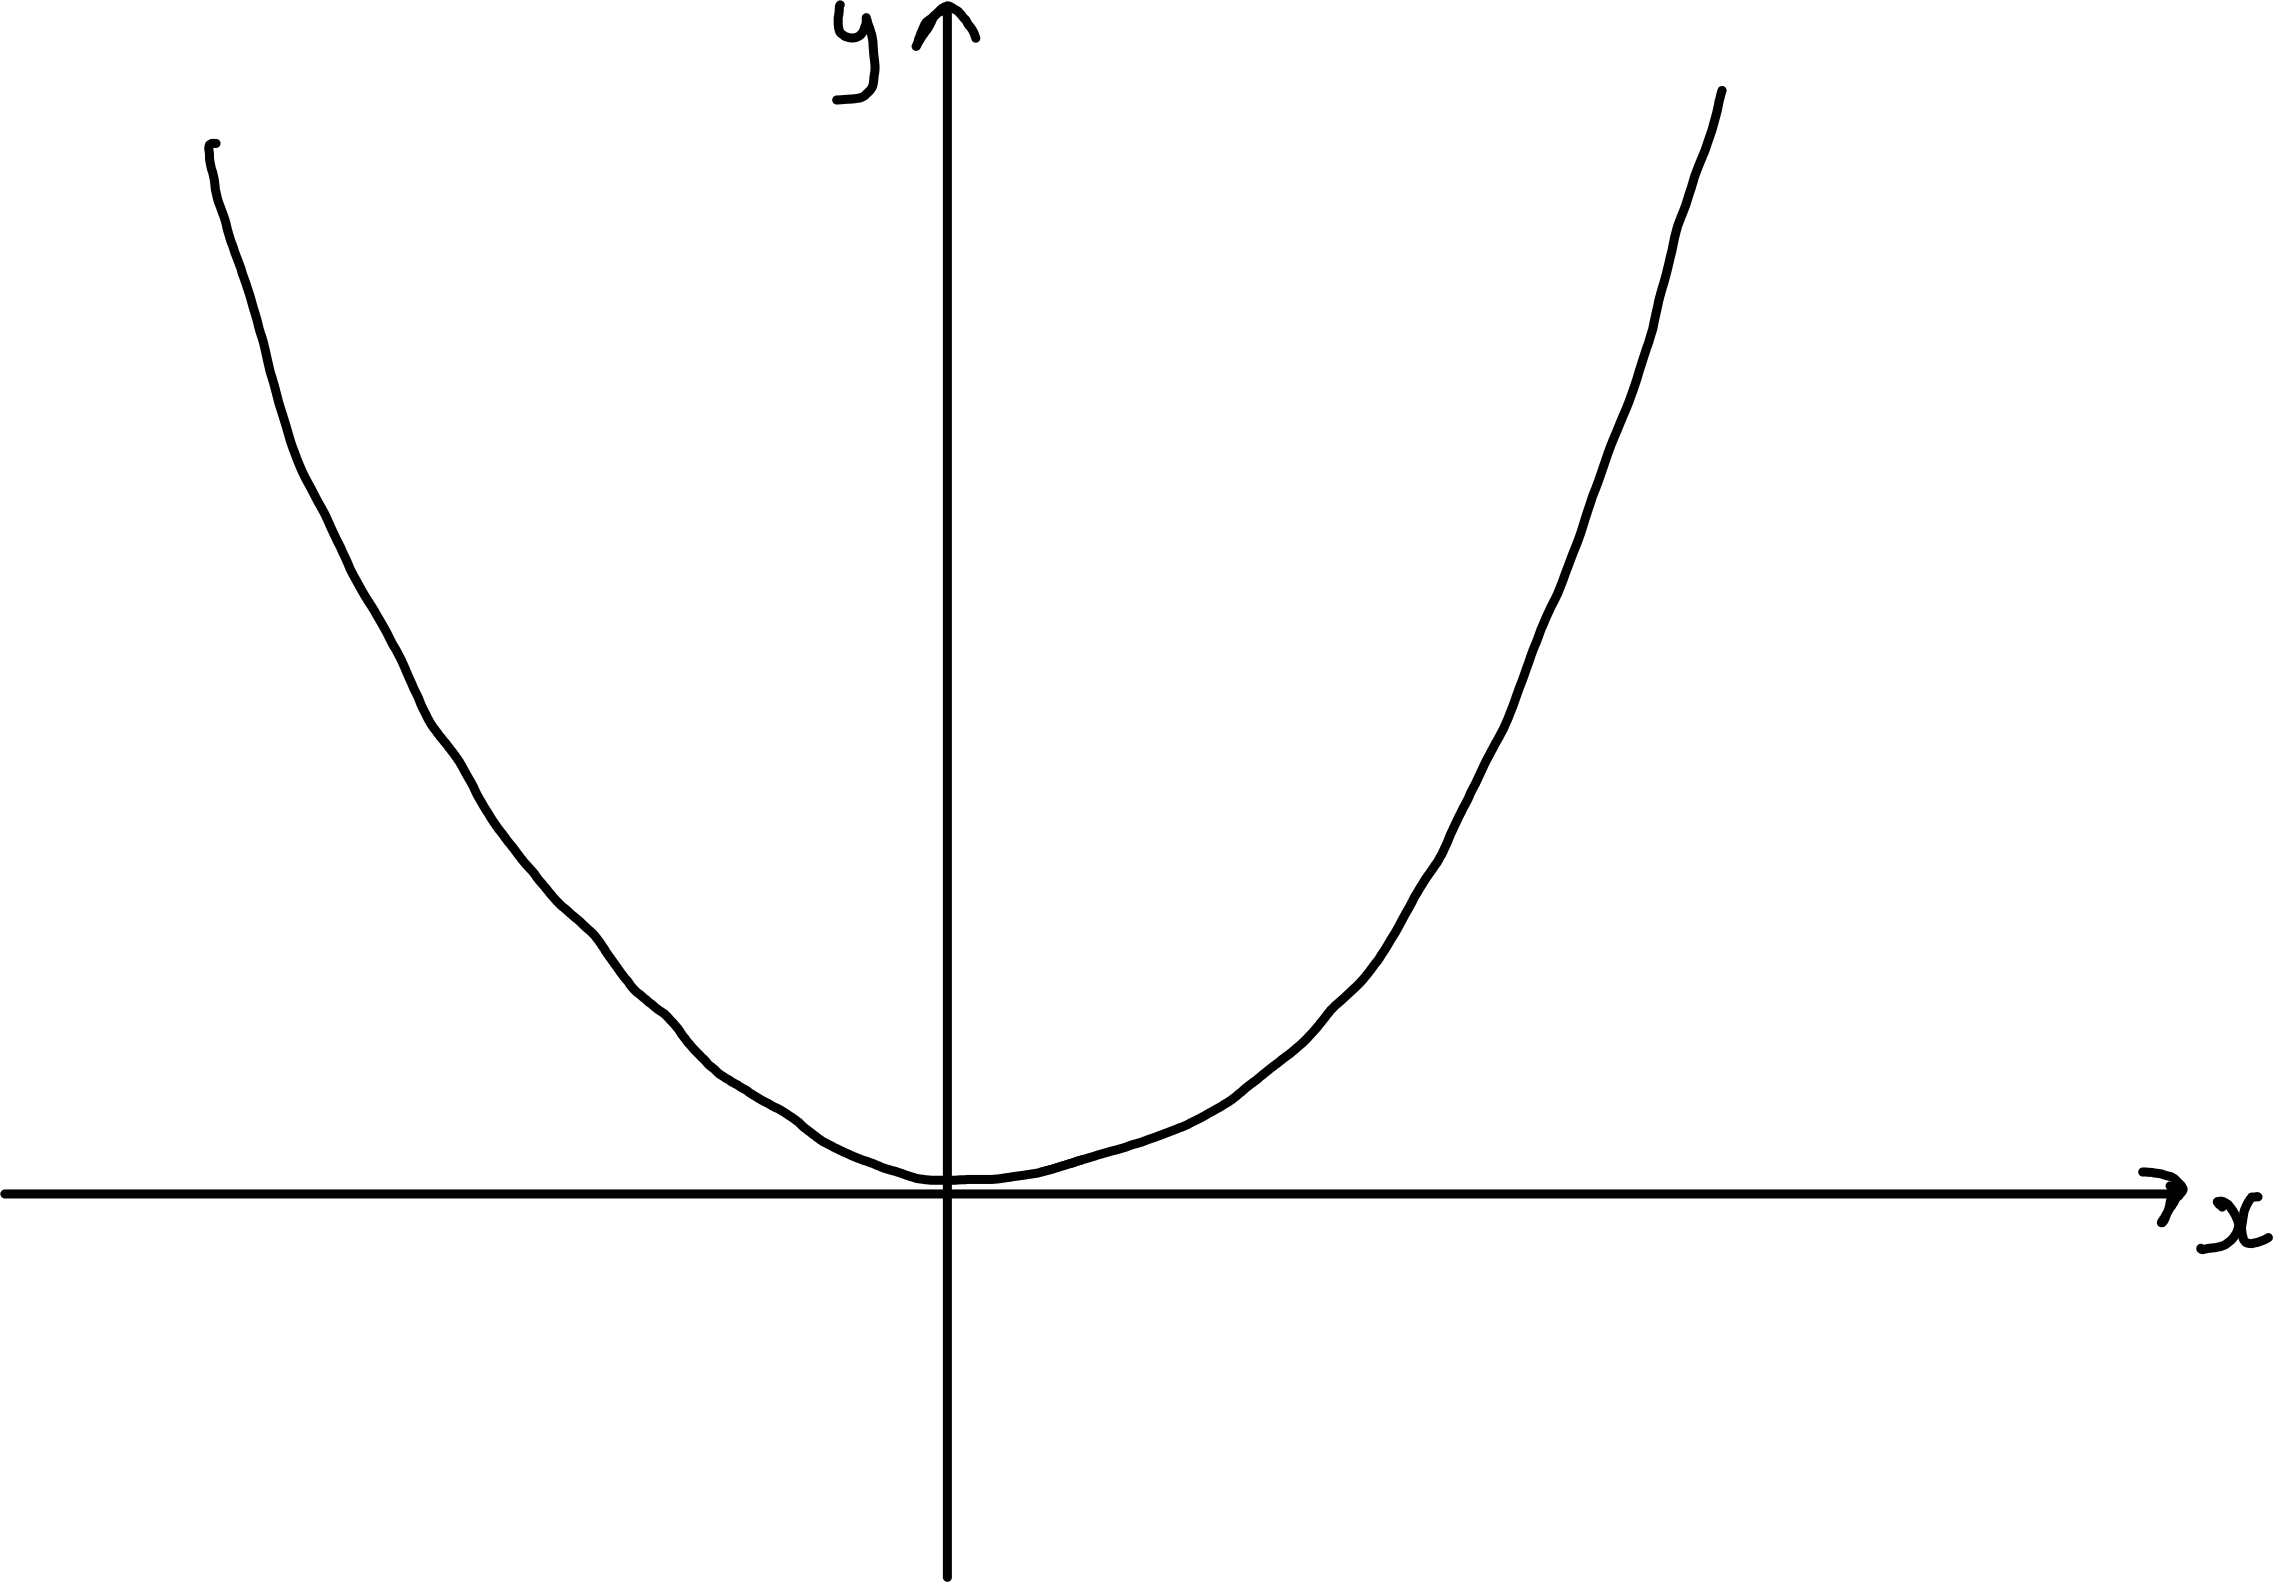
\includegraphics[height=5cm]{01-uniformcts} 
    \par}
    We want some function that looks like this, a continuous function which gets steeper as we go to infinity.
    So $f(x) = x^2$ ought to work.
    We know $f$ is cts (as it's a poly).
    Suppose $\delta > 0$.
    Then \begin{align*}
        f(x + \delta) - f(x) &= (x + \delta)^2 - x^2 \\
        &= 2 \delta x + \delta^2 \to \infty \text{ as } x \to \infty.
    \end{align*} 
    So in particular, $\forall \; \delta > 0 \ \exists \; x, y \in \mathbb{R}$ s.t. $|x-y| < \delta$ but $|f(x) - f(y)| \geq 1$.
    So conditions for uniform cty fails for $\epsilon = 1$.
    So $f$ not uniform cty.
\end{example} 

\begin{example} \label{exm:1/x}
    Make domain bounded.
    We can still fail, e.g. $f: (0, 1) \to \mathbb{R}$ cts but not uniform cts.

    { \par
    \centering 
    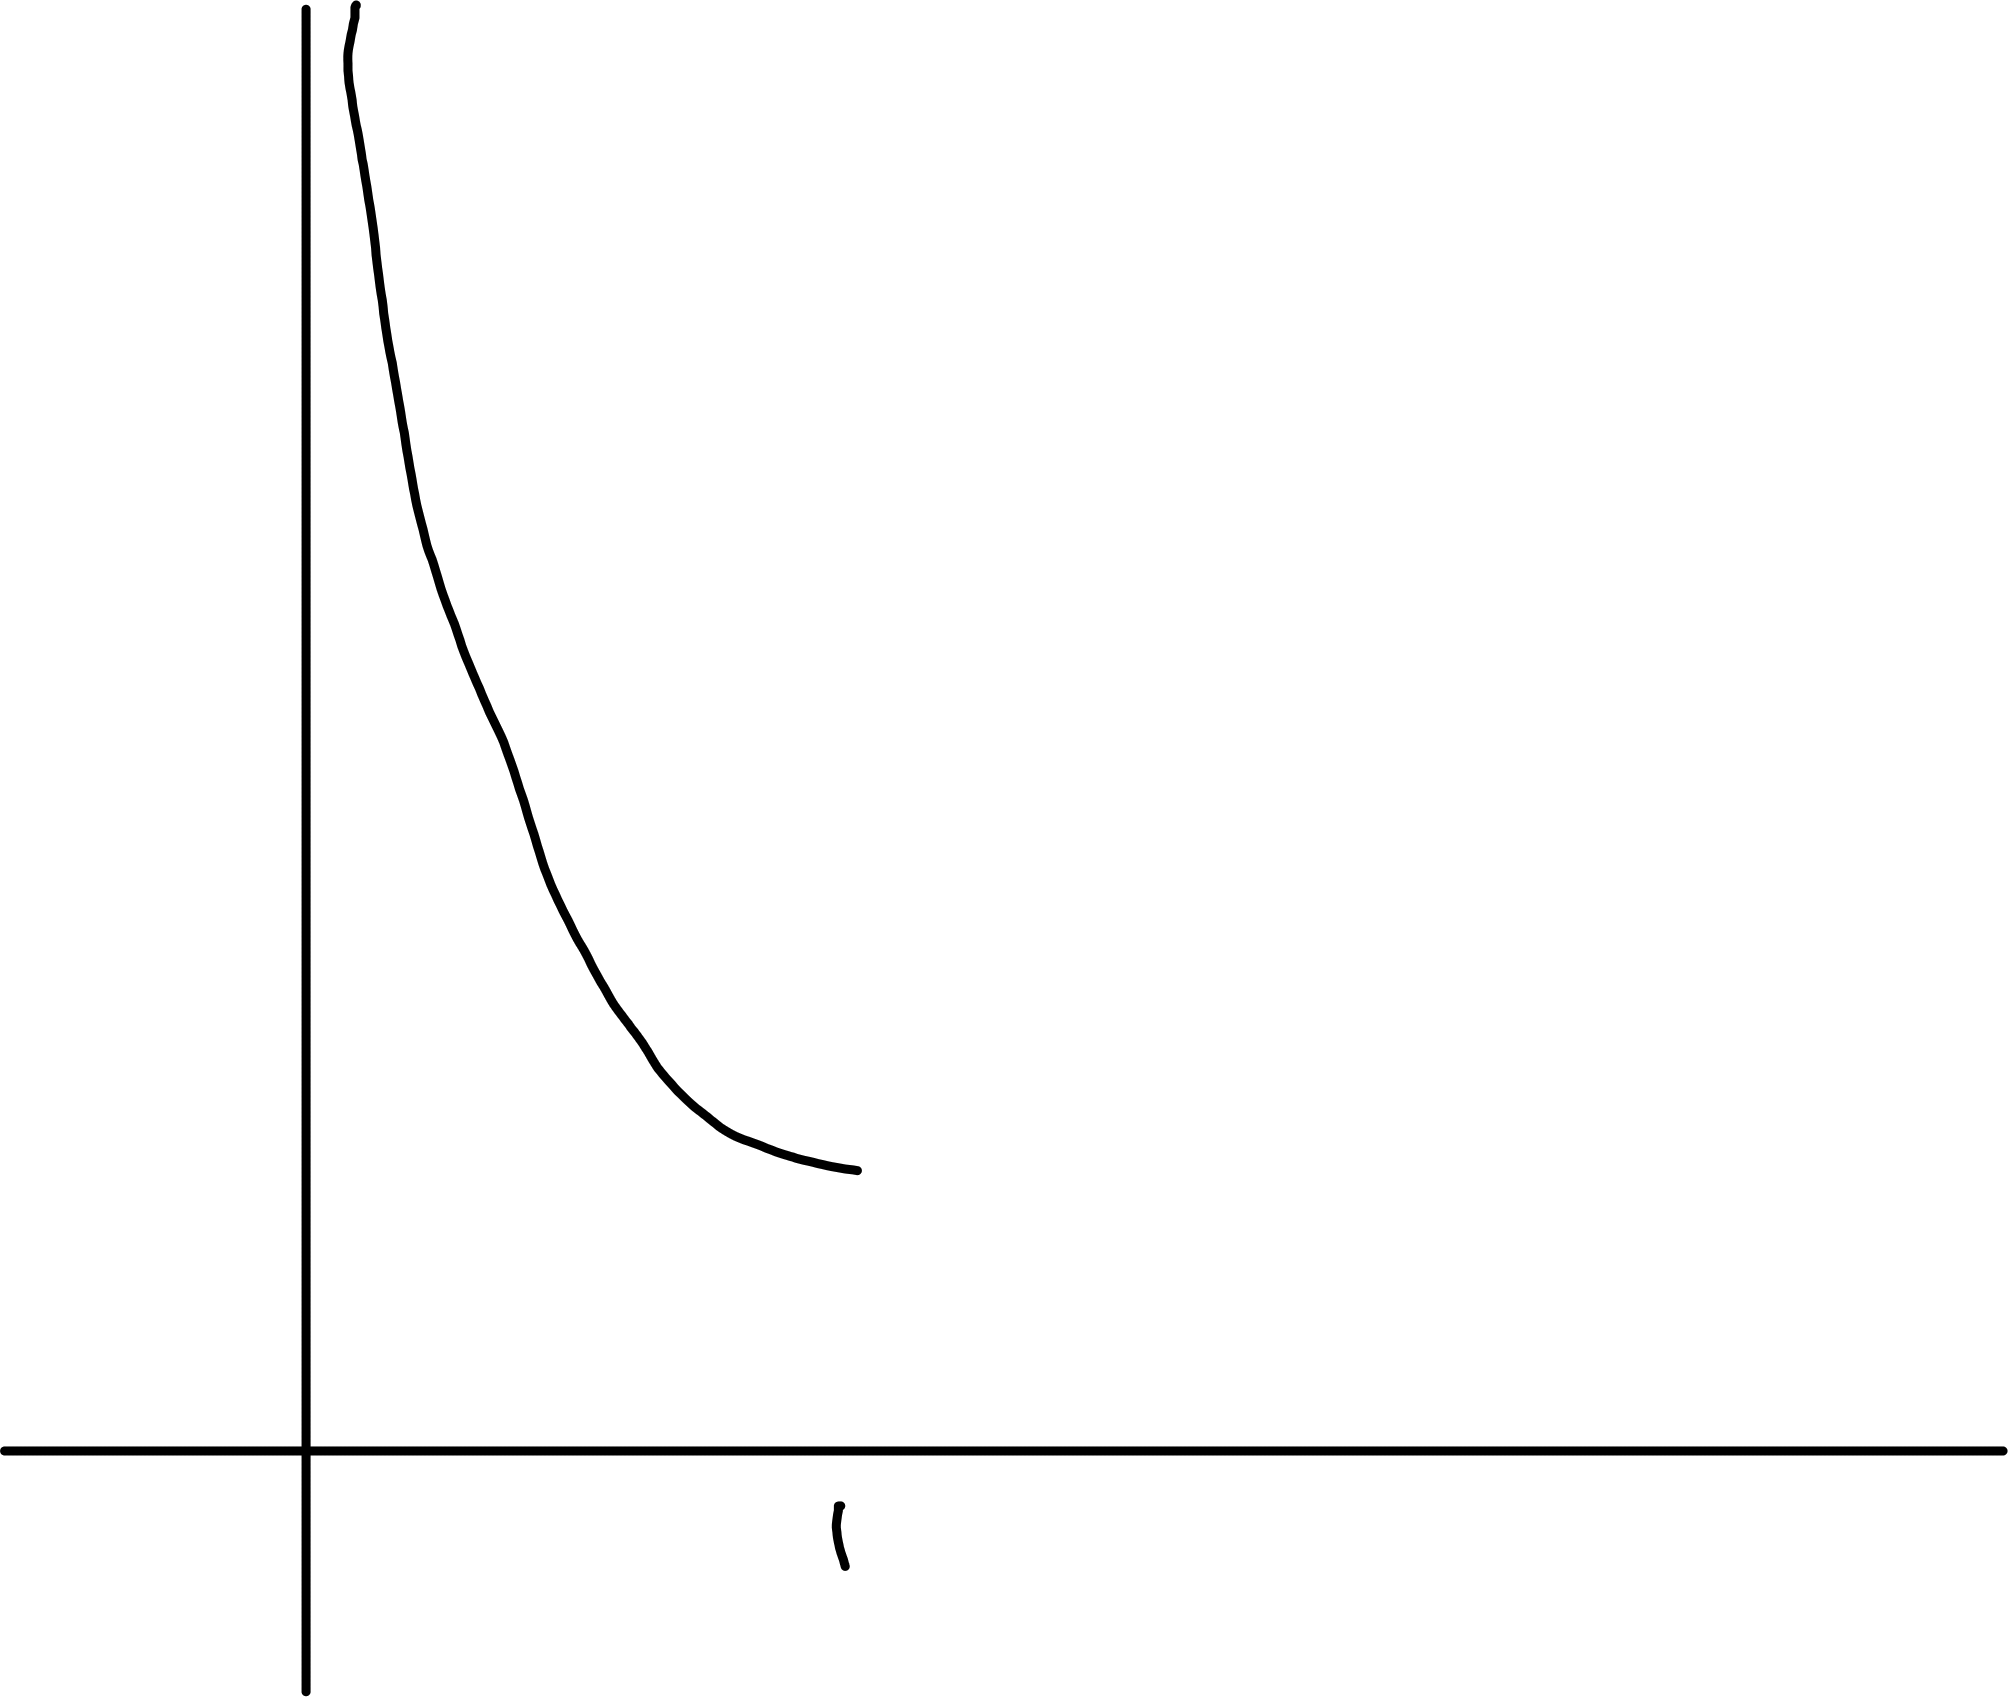
\includegraphics[height=5cm]{01-uniformcty2} 
    \par}

    Let $f(x) = \frac{1}{x}$, clearly cts.
    Proof that its not uniform continuity is left as an exercise to the reader.
\end{example} 

\begin{theorem} \label{thm:12}
    A continuous real-valued function on a closed bounded interval is uniformly continuous.
\end{theorem} 

\begin{proof}
    Let $f: [a, b] \to \mathbb{R}$ and suppose $f$ is cts but not uniformly cts. Then we can find $\epsilon > 0$ st. $\forall \; \delta > 0 \ \exists \; x,y \in [a, b]$ with $|x-y| < \delta$ but $|f(x) - f(y)| \geq \epsilon$.

    In particular, taking $\delta = \frac{1}{n}$ we can find sequences $(x_n), (y_n) \in [a, b]$ with, for each $n$, $|x_n - y_n| < \frac{1}{n}$ but $|f(x_n) - f(y_n)| \geq \epsilon$.
    The sequence $(x_n)$ is bounded so by BW\footnote{Bolzano Weierstrass} it has a convergent subsequence $x_{n_j} \to x$.
    And $[a, b]$ is a closed interval so $x \in [a, b]$.
    Then $x_{n_j} - y_{n_j} \to 0$ so $y_{n_j} \to x$.

    But $f$ is cts at $x$ so $\exists \; \delta > 0$ s.t. $\forall \; y \in [a, b]$ $|y-x| < \delta \implies |f(y) - f(x)| < \frac{\epsilon}{2}$. 
    Take such a $\delta$.
    As $x_{n_j} \to x$ we can find $J_1$ s.t. $j \geq J_1 \implies |x_{n_j} - x| < \delta$.
    Similarly we can find $J_2$ s.t. $j \geq J_2 \implies |y_{n_j} - x| < \delta$.
    Now let $j = \max (J_1, J_2)$ then $|x_{n_j} - x|, |y_{n_j} - x| < \delta$ so we have $|f(x_{n_j}) - f(x)|, |f(y_{n_j}) - f(x)| < \epsilon / 2$.
    Then $|f(x_{n_j}) - f(y_{n_j})| \leq |f(x_{n_j}) - f(x)| + |f(y_{n_j}) - f(x)| < \epsilon$ \Lightning.
\end{proof} 

\begin{corollary} \label{cor:13}
    A continuous real-valued function on a closed bounded interval is bounded.
\end{corollary} 

\begin{proof}
    Let $f:[a, b] \to \mathbb{R}$ be a continuous function, and so uniformly continuous by \cref{thm:12}.
    Then we can find $\delta > 0$ s.t. $\forall \; x, y \in [a, b] \ |x - y| < \delta \implies |f(x) - f(y)| < 1$.

    Let $M = \lceil \frac{b - a}{\delta} \rceil$.
    Let $x \in [a, b]$.
    We can find $a = x_0 \leq x_1 \leq \dots \leq x_M = x$ with $|x_i - x_{i - 1}| < \delta$ for each $i$.
    Hence
    \begin{align*}
        |f(x)| &= \qty| f(a) + \sum_{i=1}^{M} f(x_i) - f(x_{i - 1}) |\\
        &\leq |f(a)| + \sum_{i=1}^{M} |f(x_i) - f(x_{i-1})| \\
        &< |f(a)| + \sum_{i=1}^{M} 1 \\
        &= |f(a)| + M.
    \end{align*} 
\end{proof}

\begin{remark}
    Referring back to \cref{exm:1/x}, starting at $x = 1$ and going towards $x  = 0$ we can that $\delta$ gets smaller and smaller s.t. you require an infinite number of steps to get $0$.
    So $M = \infty$ essentially.
\end{remark} 

\begin{corollary} \label{cor:14}
    A continuous real-valued function on a closed bounded interval is integrable.
\end{corollary} 

\begin{proof}
    Let $f:[a, b] \to \mathbb{R}$ be a continuous function, and so uniformly continuous by \cref{thm:12}.
    Let $\epsilon > 0$.
    Then we can find $\delta > 0$ s.t. $\forall \; x, y \in [a, b] \ |x - y| < \delta \implies |f(x) - f(y)| < \epsilon$.
    Let $\mathcal{D} = \{ x_0 < x_1 < \dots < x_n\}$ be a dissection s.t. for each $i$ we have $x_i - x_{i-1} < \delta$.

    Let $i \in \{1, \dots, n\}$.
    Then for any $u, v \in [x_{i-1}, x_i]$ we have $|u - v| < \delta$ so $|f(u) - f(v)| < \epsilon$.
    Hence 
    \begin{align*}
        \sup_{x \in [x_{i-1}, x_i]} f(x) - \inf_{x \in [x_{i-1}, x_i]} f(x) \leq \epsilon.
    \end{align*} 
    Hence:
    \begin{align*}
        S(f, \mathcal{D}) - s(f, \mathcal{D}) &= \sum_{i=1}^{n} (x_i - x_{i-1}) \qty(\sup_{x \in [x_{i-1}, x_i]} f(x) - \inf_{x \in [x_{i-1}, x_i]} f(x)) \\
        &\leq \sum_{i=1}^{n} (x_i - x_{i - 1}) \epsilon \\
        &= \epsilon \sum_{i=1}^{n} (x_i - x_{i - 1}) \\
        &= \epsilon (b - a).
    \end{align*} 
    But $\epsilon(b-a)$ can be made arbitrarily small by taking $\epsilon$ small.
    So by Riemann's criterion $f$ is integrable over $[a, b]$.
\end{proof} 